\subsection{Ca sử dụng tải ảnh lên}

\vspace{0.5cm}

\noindent 
\begin{tabularx}{\linewidth}{| l | X |} 
\hline 
\textbf{Mô tả} & Người dùng tải ảnh lên để hệ thống tự động gán nhãn cho ảnh. \\
\hline 
\textbf{Luồng cơ bản} & 1. Người dùng truy cập màn hình tải ảnh lên\newline
                       2. Người dùng chọn ảnh muốn tải lên trong máy.\newline
                       3. Người dùng submit danh sách ảnh vừa chọn. \newline
                       4. Hệ thống tải ảnh lên server ảnh và gán nhãn. \newline
                       5. Hệ thống hiển thị kết quả gán nhãn ảnh. \\
\hline 
\textbf{Luồng thay thế} &
                       - Người dùng không chọn ảnh và hệ thống không cho phép submit. \\ 
\hline 
\textbf{Tiền điều kiện} & - Người dùng đăng ký / đăng nhập tài khoản thành công và hoàn thành điền form thông tin cơ bản. \\
\hline 
\textbf{Hậu điều kiện} & - Danh sách ảnh người dùng được tải lên và cập nhật vào thư viện người dùng. \\
\hline 
\textbf{Yêu cầu phi chức năng} & Hệ thống xử lý gán nhãn trên 1 ảnh không quá 2s \\
\hline 
\end{tabularx}

\vspace{0.8cm}

\noindent 
\begin{tabular}{| c | c |}
    \hline
    \textbf{Biểu đồ hoạt động} & \textbf{Quan hệ} \\ 
    \hline
    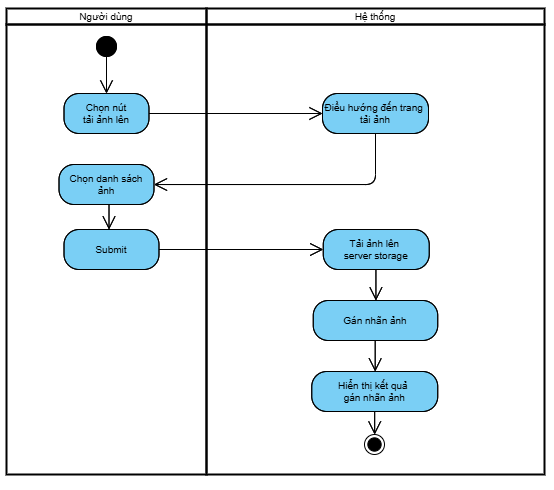
\includegraphics[width=0.6\linewidth]{figures/c3/3-3-4-activity-diagram.png} 
    & 
    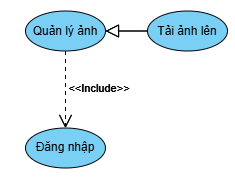
\includegraphics[width=0.35\linewidth]{figures/c3/3-3-4-relationship.png} \\ 
    \hline
\end{tabular}

\begin{figure}[H]
    \centering  
    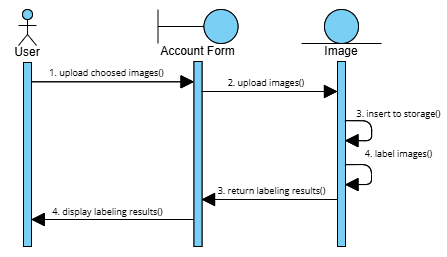
\includegraphics[width=1\textwidth]{figures/c3/3-3-4-sequence-diagram.png}
    \caption{Biểu đồ tuần tự ca sử dụng tải ảnh lên.}
    \label{fig:3-3-4-sequence-diagram}
\end{figure}